\documentclass[conference]{IEEEtran}
\usepackage[utf8]{inputenc}
\usepackage{cite}
\usepackage{amsmath}
\usepackage{amssymb}
\usepackage{graphicx}
\usepackage{hyperref}
\usepackage{booktabs}
\usepackage{float}
\usepackage{listings}
\usepackage{xcolor}
\usepackage{multirow}

% Code listing configuration
\lstset{
    basicstyle=\ttfamily\small,
    breaklines=true,
    commentstyle=\color{gray},
    keywordstyle=\color{blue},
    stringstyle=\color{red},
    showstringspaces=false,
    tabsize=4,
    captionpos=b
}

\title{Curia-Lite: Minimizing Model Size for Keyword and Temporal Query Extraction}

\author{
    \IEEEauthorblockN{Will Adair}
    \IEEEauthorblockA{University of Nebraska -- Lincoln\\
    Email: wadair2@huskers.unl.edu}
    \and
    \IEEEauthorblockN{Will Glover}
    \IEEEauthorblockA{University of Nebraska -- Lincoln\\
    Email: wglover2@huskers.unl.edu}
    \and
    \IEEEauthorblockN{Rishi Krishna}
    \IEEEauthorblockA{University of Nebraska -- Lincoln\\
    Email: rkrishna2@huskers.unl.edu}
    \and
    \IEEEauthorblockN{Michael Dejournett}
    \IEEEauthorblockA{University of Nebraska -- Lincoln\\
    Email: mdejournett2@huskers.unl.edu}
    \and
    \IEEEauthorblockN{Amy Nguyen}
    \IEEEauthorblockA{University of Nebraska -- Lincoln\\
    Email: anguyen105@huskers.unl.edu}
    \and
    \IEEEauthorblockN{Maya Wilson}
    \IEEEauthorblockA{University of Nebraska -- Lincoln\\
    Email: mwilson75@huskers.unl.edu}
    \and
    \IEEEauthorblockN{Krishnaraj Ganesan}
    \IEEEauthorblockA{University of Nebraska -- Lincoln\\
    Email: krishnarajganesan@nebraska.edu}
}

\begin{document}

\maketitle

\begin{abstract}
Curia is a campus event search system for University of Nebraska--Lincoln that parses natural-language queries into keywords and structured temporal bounds. This paper studies how far the underlying language model can be reduced while preserving keyword expansion and temporal grounding under tight CPU latency and memory budgets.

We evaluate seven model candidates---a remote 27B reference (Gemini), a local 8B baseline (Ollama llama3), and five Hugging Face models (248M--1.5B)---on two 72-query benchmarks: a temporal grounding suite and a perturbation-robustness suite. All runs use a CUDA-backed local evaluation harness to isolate model capacity from hardware variation; CPU-constrained deployment is the target environment. On the temporal suite, Gemini achieves perfect extraction (100\% parse, 100\% date and time exact-match). Among local models, Ollama llama3 (8B) parses all queries but attains only 23.61\% date exact-match at roughly 3.6\,s mean latency; Qwen 1.5B matches Gemini on date exact-match and reaches 93.75\% time exact-match at lower latency. The two T5-family encoder-decoder models return structurally valid outputs but no correct temporal fields, indicating a task-specific capacity threshold near 1\,B parameters. On the robustness suite, Gemini degrades to 25\% parse success due to endpoint sensitivity, while Qwen-family local models remain gate-stable, underscoring that robustness cannot be assumed from raw parameter count alone.
\end{abstract}

\begin{IEEEkeywords}
    Lightweight Models, Temporal Grounding, Information Retrieval, Query Parsing, Edge Inference
\end{IEEEkeywords}

\section{Introduction}
\label{sec:intro}

Curia's natural language search system depends on two query-understanding capabilities: extracting and expanding intent-bearing keywords for retrieval, and grounding temporal expressions into structured date and time bounds. A user typing ``free food next Thursday after 3pm'' has simultaneously specified a topic, a relative date anchor, and a time lower bound. Converting this free-form input into structured filters drives retrieval quality.

In practice, the search must operate under tight memory and latency budgets, which pushes deployment toward smaller models. This raises a central design tension: how far can the underlying model be reduced before these extraction behaviors degrade enough to harm retrieval? Prior work on neural scaling laws~\cite{kaplan2020scaling,hoffmann2022training} suggests that capabilities can decline unevenly as capacity decreases, and the effect is often amplified when the task requires reliable structured output.

This paper studies that tension directly in Curia, a campus event search system for UNL. Rather than targeting architectural novelty, we measure how model size affects the two core tasks that drive retrieval: keyword expansion and temporal grounding. We focus on four research questions:
\begin{enumerate}
    \item Does the gap between the two tasks, temporal grounding and keyword expansion, begin to diverge as model size decreases?
    \item At what point can our structured prompt no longer produce usable results?
    \item How stable are these results, and does the stability substantively change as model size decreases?
    \item What model size offers the best tradeoff among stability, accuracy, and latency?
\end{enumerate}

Our experiments show asymmetric degradation across tasks and datasets. Temporal grounding is more fragile than keyword expansion under perturbation, and performance does not scale monotonically with parameter count alone. In particular, selected mid-scale local models (specifically the Qwen-family at 0.5B and 1.5B) remain usable under the correctness gate profile on both suites, while very small models and certain endpoint-dependent configurations fail critical checks.

This paper makes three contributions:
\begin{itemize}
    \item \textbf{Task-specific size analysis}: An empirical comparison of seven model candidates (248M to 27B) on keyword expansion and temporal grounding within the same event-search pipeline, evaluated on a benchmark of 72 labeled temporal queries.
    \item \textbf{Failure characterization}: Documentation of how and where temporal extraction breaks down as model capacity decreases, showing that structured-output correctness is unrecoverable below 1B parameters through prompt engineering or fallback heuristics alone.
    \item \textbf{Deployment guidance}: Evidence that keyword expansion is more size-resilient than temporal grounding, with practical implications for feature-selection and model-selection at different deployment scales.
\end{itemize}

\section{Related Work}
\label{sec:related}

Our work sits at the intersection of neural scaling, temporal information extraction, in-context learning, and small-model deployment. We review the most relevant prior work in each area below.

\subsection{Neural Scaling Laws}

Kaplan et al.~\cite{kaplan2020scaling} showed that language model loss scales as a power law with model size, dataset size, and compute across seven orders of magnitude. Hoffmann et al.~\cite{hoffmann2022training} refined this, finding that many widely-used models are undertrained relative to their parameter count and that tokens and parameters should be scaled together. Both results bear directly on our study: if performance degrades predictably with size, we should be able to identify a parameter range where structured extraction breaks down---and our experiments show that range is sharper than a smooth power law would suggest.

\subsection{Temporal Extraction and Hybrid Retrieval}

HeidelTime~\cite{strotgen2010heideltime} is a rule-based system for extracting and normalizing temporal expressions using hand-crafted grammars. It works well on standard patterns but needs domain-specific tuning for new text types. We use \texttt{dateparser} in a similar capacity as a fallback: when the LLM returns malformed JSON, it tries to recover any parseable date strings. The catch is that it only fires on parse failures---when the model returns valid JSON with wrong dates, which is the main failure we document, the fallback never gets a chance to run. For keyword expansion, Reimers and Gurevych~\cite{reimers2019sentencebert} showed that Siamese BERT networks produce dense sentence embeddings well-suited for semantic similarity search. We use \texttt{all-MiniLM-L6-v2}, a compact Sentence-BERT model, to retrieve semantically related domain terms and append them to the LLM's keyword output at under 50\,ms per query.

\subsection{Few-Shot and In-Context Learning}

Brown et al.~\cite{brown2020language} showed that large language models can follow new task specifications from a handful of in-context examples alone, no weight updates needed, and that this ability improves with scale. We rely on this throughout: all models receive the same in-context exemplars (4 temporal, 3 keyword) under an identical prompt contract. Our results quantify the scale dependency: the 27B Gemini reference reliably produces correct temporal bounds across the suite, while local models show heterogeneous behavior. The Qwen 1.5B run achieves parity with Gemini on strict date exact-match, whereas the Ollama 8B baseline attains modest strict-date performance (23.61\%) and moderate time accuracy (39.58\%). Several smaller candidates fail to produce consistent temporal bounds, suggesting a capacity threshold for dependable structured temporal grounding under CPU-constrained execution.

\subsection{Small and Specialized Language Models}

Several groups have looked at whether small models are viable substitutes for large ones in narrow domains. Grangier et al.~\cite{grangier2024small} propose resampling pretraining data toward a target domain using importance sampling, alongside a projected-network architecture that compresses a large model into a smaller one at inference time. Belcak et al.~\cite{belcak2025slm} make the broader argument that SLMs are a natural fit for the repetitive, single-purpose subtasks that show up in production agentic pipelines. Fan et al.~\cite{fan2025smallmighty} report that sub-3B models can compete on time-series forecasting when given descriptive statistical prompts and an adaptive fusion layer. These papers make a reasonable case that small models are worth taking seriously for specialized tasks. We test that idea on structured temporal grounding and find the gap to the 27B reference model is not closeable in the sub-2B range under our evaluation conditions.

\section{Methodology}
\label{sec:method}

\subsection{Evaluation Design}

The benchmark is structured as a fixed evaluation matrix over a predefined model set and two dataset presets. The model matrix includes seven candidates: a Gemini reference (27B remote), a local Ollama baseline (8B), and five Hugging Face models (248M--1.5B). The primary evaluation dataset is \texttt{rigorous-temporal}, a 72-query benchmark focused on temporal grounding with labeled date/time bounds. A secondary \texttt{rigorous-robustness} dataset of 72 perturbed queries tests stability under adversarial and edge-case phrasing; both datasets are evaluated in the main results. The \texttt{all-events} preset covering the full event catalog exceeds 10 hours on consumer machines and is excluded to prioritize reproducibility.

The protocol keeps the inference backend and execution mode explicit. All runs use the local Hugging Face backend on CUDA GPU to ensure consistent, hardware-isolated latency comparisons; CPU-constrained deployment is the intended production environment. The benchmark measures the interaction between model capacity and the Curia query-understanding pipeline under a stable test harness, permitting clean attribution of performance differences to model scale rather than implementation variation.

\subsection{Task Outputs}

Given a natural language query $q$, Curia produces two outputs:
\begin{itemize}
    \item \textbf{Keywords}: An expanded set of intent-bearing terms for retrieval matching.
    \item \textbf{Temporal bounds}: A JSON object with four fields — \texttt{date\_from}, \texttt{date\_to}, \texttt{time\_from}, \texttt{time\_to} — or \texttt{null} when no constraint is present.
\end{itemize}

For example, ``morning concerts next weekend'' should yield:
\begin{lstlisting}[language={}]
{
  "date_from": "2026-05-02",
  "date_to":   "2026-05-03",
  "time_from": "06:00",
  "time_to":   "12:00",
  "keywords":  ["concert", "music",
                "performance", "band", "show"]
}
\end{lstlisting}

\subsection{Scoring Framework}

The correctness suite summarizes each model with task-level extraction metrics. For a query $q$, the benchmark records whether the model returns parseable JSON, whether the date and time fields match the labeled targets, and whether the predicted keywords align with the expected keyword set. The reported metrics are: parse success rate, date exact-match rate, time exact-match rate (temporal suite) or time partial-match rate (robustness suite), and keyword F1.

Keyword F1 and parse success are always computed over all 72 queries. Date and time rates are computed over their respective labeled subsets: the temporal dataset has 72 date-labeled and 48 time-labeled queries; the robustness dataset has 48 date-labeled and 24 time-labeled queries. Percentage rates reported in tables therefore have different effective denominators depending on the column. On the robustness suite, no model achieves nonzero time exact-match (the robustness queries target partial rather than strict time alignment), so we report time partial-match in Table~\ref{table:robustness_accuracy} instead.

A binary correctness gate determines overall model usability with thresholds: parse $\geq 0.70$, keyword F1 $\geq 0.05$, date exact $\geq 0.50$, and time partial $\geq 0.50$. A model passes only if all four criteria are met. The goal of these gates is to identify models that remain deployable under minimum service-level requirements; results near the threshold boundaries are noted where relevant.

The central analytical question is whether keyword expansion and temporal grounding degrade together as model size decreases, or diverge. A model that retains strong keyword F1 but fails date extraction, or vice versa, indicates that the two capabilities have different capacity thresholds---a finding that has direct implications for feature selection at deployment.

\subsection{Inference Paths}

\paragraph{Gemini Remote Path (27B baseline)}
The reference path sends a single structured prompt to \texttt{gemma-3-27b-it} via the \texttt{google-genai} SDK. The prompt includes the current date and requests a JSON object containing temporal fields, keyword expansion, and retrieval-oriented output. This path serves as the upper-bound reference for quality-versus-latency comparisons and gate-pass analysis reported in the evaluation.

\paragraph{Local Model Path}
The local HuggingFace candidates execute with automatic device selection: CUDA when available, falling back to CPU otherwise. The Ollama baseline (llama3:latest) runs through Ollama's local inference server. Each model is evaluated with the same structured prompt contract, the same top-level output schema, and the same decoding settings so that differences in output quality are attributable to model capacity rather than prompt redesign. The benchmark runner preserves a fixed prompt interface across all local candidates; the only variation is the model identity and the execution backend.

\paragraph{Fallback Layer}
For malformed JSON outputs, the benchmark applies a fallback policy: (1) attempt \texttt{dateparser} to recover parseable date strings when JSON parsing fails; (2) time-of-day keyword lookup for time fields (morning $\to$ 06:00--12:00, afternoon $\to$ 12:00--17:00, evening $\to$ 17:00--21:00); (3) null bounds if both fail. This recovery layer applies uniformly across all models, allowing divergence in performance to be attributed to model capacity. However, the fallback only recovers from malformed JSON; when a model returns valid JSON with incorrect temporal values (e.g., wrong date arithmetic), the fallback does not intervene, and the error is recorded as-is in the results.

% MiniLM subsection removed; model not part of evaluated matrix

\subsection{Event Scoring}

The backend ranks events by weighted field score:
\[
\text{score}(e, Q) = \sum_{t \in Q} w_f \cdot \mathbf{1}[t \in \text{field}_f(e)] \cdot \text{pos}(t, Q)
\]
where $w_f \in \{4, 2, 1\}$ for name, venue/category, and description/tags respectively, and $\text{pos}(t,Q)$ is a position bonus giving higher weight to terms that appear earlier in the query. Temporal bounds are applied as hard pre-filters before scoring.

\subsection{Models Evaluated}

Table~\ref{table:models} lists the seven model candidates evaluated in the benchmark harness.

\begin{table}[ht]
    \centering
    \caption{Model Candidates}
    \resizebox{\columnwidth}{!}{%
    \begin{tabular}{llr}
        \toprule
        \textbf{Model} & \textbf{Backend} & \textbf{Params} \\
        \midrule
        \texttt{gemma-3-27b-it} & Gemini API & 27B \\
        \texttt{llama3:latest} & Ollama local & 8B \\
        \texttt{Qwen2.5-0.5B} & HF local & 500M \\
        \texttt{Qwen2.5-1.5B} & HF local & 1.5B \\
        \texttt{TinyLlama-1.1B-Chat} & HF local & 1.1B \\
        \texttt{google/flan-t5-base} & HF local & 250M \\
        \texttt{LaMini-Flan-T5-248M} & HF local & 248M \\
        \bottomrule
    \end{tabular}}
    \label{table:models}
\end{table}

\subsection{Model Selection Rationale}

The benchmark model set was selected to probe the parameter-performance frontier at key intervals and to include both instruction-tuned decoder-only and encoder-decoder architectures. \texttt{gemma-3-27b-it} serves as the remote reference model---a production-grade instruction-tuned 27B decoder-only model via the Gemini API that reliably solves both tasks. \texttt{llama3:latest} (8B) is included as a local baseline available via Ollama, bridging between the Gemini scale and smaller local candidates while remaining practical for CPU inference.

The local decoder-only candidates span the sub-1B region: \texttt{Qwen2.5-0.5B} (500M, instruction-tuned, chat-templated) is the active default in production due to its speed and performance on lower-range consumer machines; \texttt{Qwen2.5-1.5B} (1.5B, same architecture) was included to test whether crossing into the 1B range improves temporal reasoning at the cost of latency; and \texttt{TinyLlama-1.1B-Chat} (1.1B, a multi-turn chat-optimized model) was included to evaluate whether alternative chat architectures in the 1B range escape the structured-output ceiling. The encoder-decoder candidates are smaller T5 variants: \texttt{flan-t5-base} (250M, instruction-tuned via FLAN) and \texttt{LaMini-Flan-T5-248M} (248M, a distilled T5 trained for abstractive tasks). These were included to determine whether the seq2seq inductive bias offers advantages over decoder-only scaling for this task.

\section{Results}
\label{sec:results}

\subsection{Benchmark Design}

We evaluate the same seven-model matrix on two 72-case correctness datasets: \texttt{rigorous-temporal} and \texttt{rigorous-robustness}. The temporal set emphasizes explicit temporal grounding, while the robustness set introduces perturbed/edge query forms. Both runs use the same prompt contract, decoding settings, and CUDA local backend configuration where applicable.

All numeric values in this section are taken directly from the synced artifacts under \texttt{figures/correctness/temporal/data/} and \texttt{figures/correctness/robustness/data/} (\texttt{summary.json} and \texttt{gate\_results.json}). End-to-end retrieval metrics (top-$N$ event hit rate, MRR) are recorded in the run artifacts but are all zero across both datasets and all models, because the events corpus was not available in the evaluation environment; only extraction metrics are reported here.

\subsection{Accuracy on the Temporal Dataset}

Table~\ref{table:temporal_accuracy} reports the canonical extraction metrics computed from the benchmark run artifacts. Parse success is the fraction of queries returning valid JSON; keyword F1 is the overlap between predicted and expected keyword sets; both are aggregated over all 72 queries. Date exact-match is also over all 72 date-labeled queries. Time exact-match is computed over the 48 queries that carry time labels (the remaining 24 have no expected time constraint); percentages in that column therefore have an effective denominator of 48.

\begin{table*}[t]
    \centering
    \caption{Temporal Correctness Suite: Extraction Accuracy (72 queries). Date exact over 72 labeled cases; Time Exact over 48 time-labeled cases; KW F1 and Parse over all 72.}
    \begin{tabular}{lcccccr}
        \toprule
        \textbf{Model} & \textbf{Params} & \textbf{Parse} & \textbf{Date Exact} & \textbf{Time Exact} & \textbf{KW F1} & \textbf{Mean Latency (ms)} \\
        \midrule
        \texttt{gemma-3-27b-it} (Gemini)    & 27B   & 100\% & 100\% & 100\% & 0.065 & 8{,}375 \\
        \texttt{llama3:latest} (Ollama)     & 8B    & 100\% & 23.61\% & 39.58\% & 0.225 & 3{,}580 \\
        \texttt{Qwen2.5-1.5B}          & 1.5B  & 100\% & 100\% & 93.75\% & 0.0626 & 2{,}896 \\
        \texttt{TinyLlama-1.1B-Chat}        & 1.1B  & 98.61\% & 98.61\% & 52.08\% & 0.167 & 2{,}120 \\
        \texttt{Qwen2.5-0.5B}          & 500M  & 94.44\% & 81.94\% & 54.17\% & 0.098 & 3{,}952 \\
        \texttt{google/flan-t5-base}        & 250M  & 86.11\% & 0\%    & 0\%    & 0.000 & 844   \\
        \texttt{LaMini-Flan-T5-248M}         & 248M  & 98.61\% & 0\%    & 0\%    & 0.000 & 853   \\
        \bottomrule
    \end{tabular}
    \label{table:temporal_accuracy}
\end{table*}

The remote Gemini reference achieves perfect extraction rates on this benchmark (100\% parse, date, and time exact-match) under the structured prompt contract used for the run. Among local candidates, the picture is heterogeneous: the Ollama 8B model parses every query but attains only 23.6\% strict date exact-match and 39.6\% time exact-match, while achieving a relatively high keyword F1 (0.225). The Qwen 1.5B run attains full date exact-match parity with Gemini and near-parity on time exact-match (93.75\%), at a lower mean latency than Gemini. Several smaller models (the two T5 variants at ~250\,M) produce no correct temporal fields on this suite despite non-trivial parse success.

\subsection{Accuracy on the Robustness Dataset}

Table~\ref{table:robustness_accuracy} summarizes the same metrics on \texttt{rigorous-robustness}. This dataset has 48 date-labeled and 24 time-labeled cases out of 72 total queries; rate denominators differ by column accordingly. We report time \emph{partial} rate rather than time exact-match because no model achieves nonzero time exact-match on this suite---the robustness queries are designed around partial time-range agreement rather than strict field equality---making time partial the operationally meaningful criterion.

\begin{table*}[t]
    \centering
    \caption{Robustness Correctness Suite: Extraction Accuracy (72 queries). Date Exact over 48 date-labeled cases; Time Partial over 24 time-labeled cases; KW F1 and Parse over all 72.}
    \begin{tabular}{lcccccr}
        \toprule
        \textbf{Model} & \textbf{Params} & \textbf{Parse} & \textbf{Date Exact} & \textbf{Time Partial} & \textbf{KW F1} & \textbf{Mean Latency (ms)} \\
        \midrule
        \texttt{gemma-3-27b-it} (Gemini)    & 27B   & 25.00\% & 25.00\% & 25.00\% & 0.0134 & 2{,}349 \\
        \texttt{llama3:latest} (Ollama)     & 8B    & 100\%   & 41.67\% & 54.17\% & 0.290  & 3{,}524 \\
        \texttt{Qwen2.5-1.5B}          & 1.5B  & 100\%   & 100\%   & 91.67\% & 0.0980 & 2{,}768 \\
        \texttt{TinyLlama-1.1B-Chat}        & 1.1B  & 100\%   & 100\%   & 95.83\% & 0.0478 & 1{,}412 \\
        \texttt{Qwen2.5-0.5B}          & 500M  & 100\%   & 97.92\% & 62.50\% & 0.0507 & 1{,}932 \\
        \texttt{google/flan-t5-base}        & 250M  & 93.06\% & 0\%     & 0\%     & 0.000  & 858   \\
        \texttt{LaMini-Flan-T5-248M}         & 248M  & 98.61\% & 0\%     & 0\%     & 0.000  & 991   \\
        \bottomrule
    \end{tabular}
    \label{table:robustness_accuracy}
\end{table*}

Relative to temporal, robustness exposes sharper degradation in temporal grounding and stronger backend sensitivity in this specific run. Notably, Gemini drops to 25\% parse success and 75\% error rate on this robustness execution, while Qwen 1.5B and Qwen 0.5B remain gate-passing under the correctness profile.

\subsection{Research Questions (RQ1--RQ4)}

\subsubsection{RQ1: Do temporal grounding and keyword expansion diverge as size decreases?}

\textbf{Determination: Yes, and the divergence is visible in both datasets.}

On \texttt{rigorous-temporal}, Ollama 8B attains the highest keyword F1 (0.225) but low strict temporal rates (23.61\% date exact, 39.58\% time exact), while Qwen 1.5B has much lower keyword F1 (0.0626) yet near-perfect temporal grounding (100\% date exact, 93.75\% time exact). On \texttt{rigorous-robustness}, the same pattern persists: Ollama again leads keyword F1 (0.290) but remains weaker in temporal grounding (41.67\% date exact, 54.17\% time partial) than Qwen 1.5B (100\% date exact, 91.67\% time partial). This indicates the two tasks do not degrade together under downscaling.

One counterintuitive result in Table~\ref{table:temporal_accuracy} is that Gemini---the 27B reference---attains the \emph{lowest} keyword F1 (0.065) of all models that successfully parse. This reflects a precision-recall mismatch: Gemini's keyword precision is 0.034 against the labeled set, while its recall (0.671) is comparable to Ollama's (0.685). Gemini over-generates a broad synonym list whose members do not overlap with the curated label vocabulary, yielding low F1 despite returning relevant terms. This is a property of the label set construction, not evidence that Gemini performs worse at keyword expansion than smaller models.

\subsubsection{RQ2: At what point does the structured prompt stop producing usable results?}

\textbf{Determination: Around the 250M class for both datasets, with additional robustness-specific failures in larger models.}

Using the correctness gates (parse $\geq 0.70$, KW F1 $\geq 0.05$, date exact $\geq 0.50$, time partial $\geq 0.50$) applied from \texttt{gate\_results.json}, temporal passes 4/7 models (Gemini, Qwen 1.5B, TinyLlama 1.1B, Qwen 0.5B), while robustness passes only 2/7 (Qwen 1.5B and Qwen 0.5B). Both T5-family models (250M and 248M) fail both datasets with 0\% date exact, 0\% time, and 0 keyword F1, indicating non-usable extraction despite mostly parseable output. In robustness, Gemini also fails (25\% parse success), showing that usability depends on both model capacity and endpoint reliability under perturbation.

Two gate outcomes are worth noting explicitly. TinyLlama-1.1B passes the temporal gate but fails on robustness---not because of temporal degradation (it achieves 100\% date exact and 95.83\% time partial on robustness) but because its keyword F1 (0.0478) falls marginally below the 0.05 threshold. This is the narrowest gate failure in the set and illustrates how a single weak dimension can disqualify an otherwise strong model. Similarly, Qwen 0.5B passes robustness with a keyword F1 of 0.0507---a margin of 0.002 above the same threshold---making both outcomes sensitive to the gate boundary.

\subsubsection{RQ3: How stable are results as size decreases?}

\textbf{Determination: Stability varies by model family; lower size does not monotonically imply lower stability, but variance spikes appear in selected small models.}

Each dataset here uses one run per query (run count = 1), so inter-run standard deviation is unavailable; we therefore use latency spread and error rates as a stability proxy. On temporal, Qwen 0.5B shows high tail latency (p50 = 2,277 ms, p95 = 16,187 ms, max = 35,293 ms), and TinyLlama shows occasional spikes (max = 27,807 ms) despite low p50. On robustness, Qwen 1.5B and Qwen 0.5B have tighter tails (p95 = 3,376 ms and 2,724 ms respectively), while Gemini exhibits instability in correctness itself (75\% error rate in this run). Thus, stability changes with model/back-end interaction rather than parameter count alone.

\subsubsection{RQ4: What model size offers the best tradeoff among stability, accuracy, and latency?}

\textbf{Determination: Qwen 1.5B is the strongest overall balanced point across both datasets; Qwen 0.5B is a latency-oriented fallback with reduced robustness margin.}

Qwen 1.5B combines high extraction quality on temporal (100\% date exact, 93.75\% time exact) and robustness (100\% date exact, 91.67\% time partial) with moderate latency (2,896 ms temporal mean; 2,768 ms robustness mean). Qwen 0.5B is faster on robustness (1,932 ms mean) and still gate-passing, but has lower temporal reliability (81.94\% date exact and 54.17\% time exact on temporal). Ollama 8B offers strong keyword F1 but does not clear date exact gates in either dataset.

\subsection{Supporting Visualizations}

\begin{figure}[ht]
    \centering
    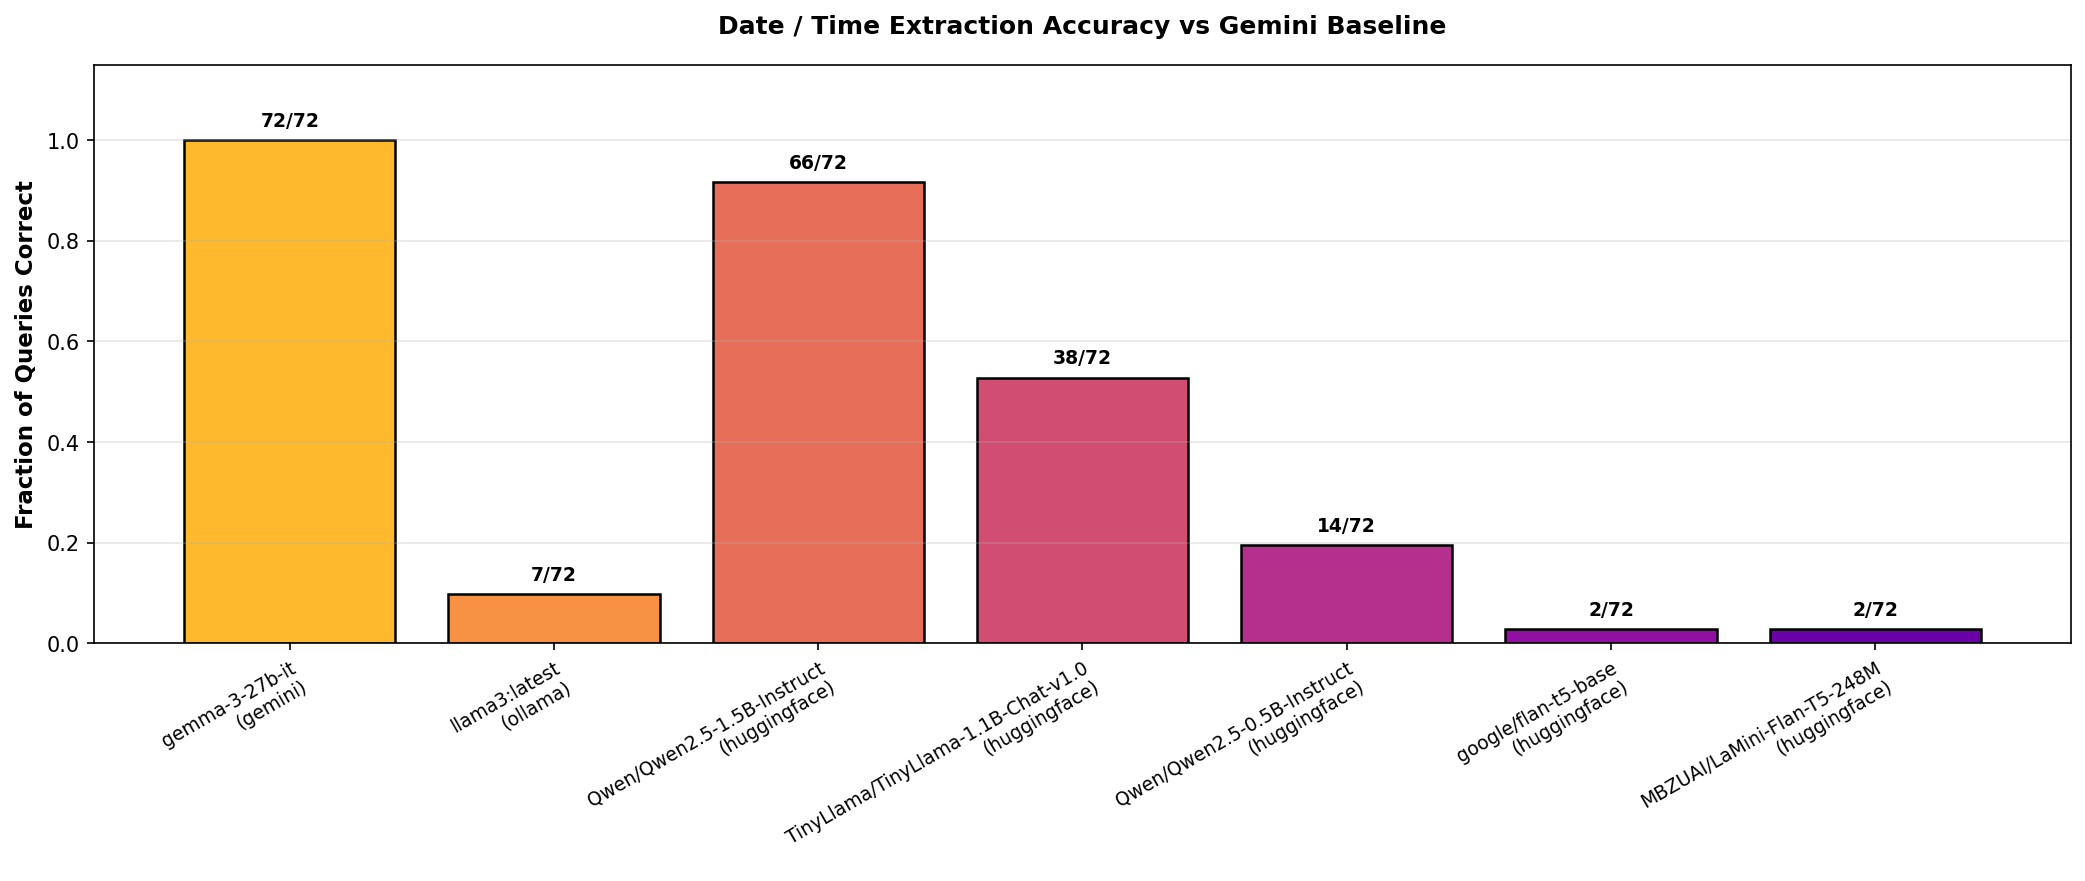
\includegraphics[width=\columnwidth]{../figures/correctness/temporal/fig1_jaccard.png}
    \caption{Temporal-suite retrieval overlap with the Gemini baseline. Each bar shows the fraction of queries on which a model's top-10 event results match Gemini's, reflecting the compounded effect of date correctness, time correctness, and keyword ranking. Models with higher date exact-match in Table~\ref{table:temporal_accuracy} correspondingly show higher overlap here; T5-family models produce zero overlap due to complete temporal extraction failure.}
    \label{fig:jaccard}
\end{figure}

\begin{figure}[ht]
    \centering
    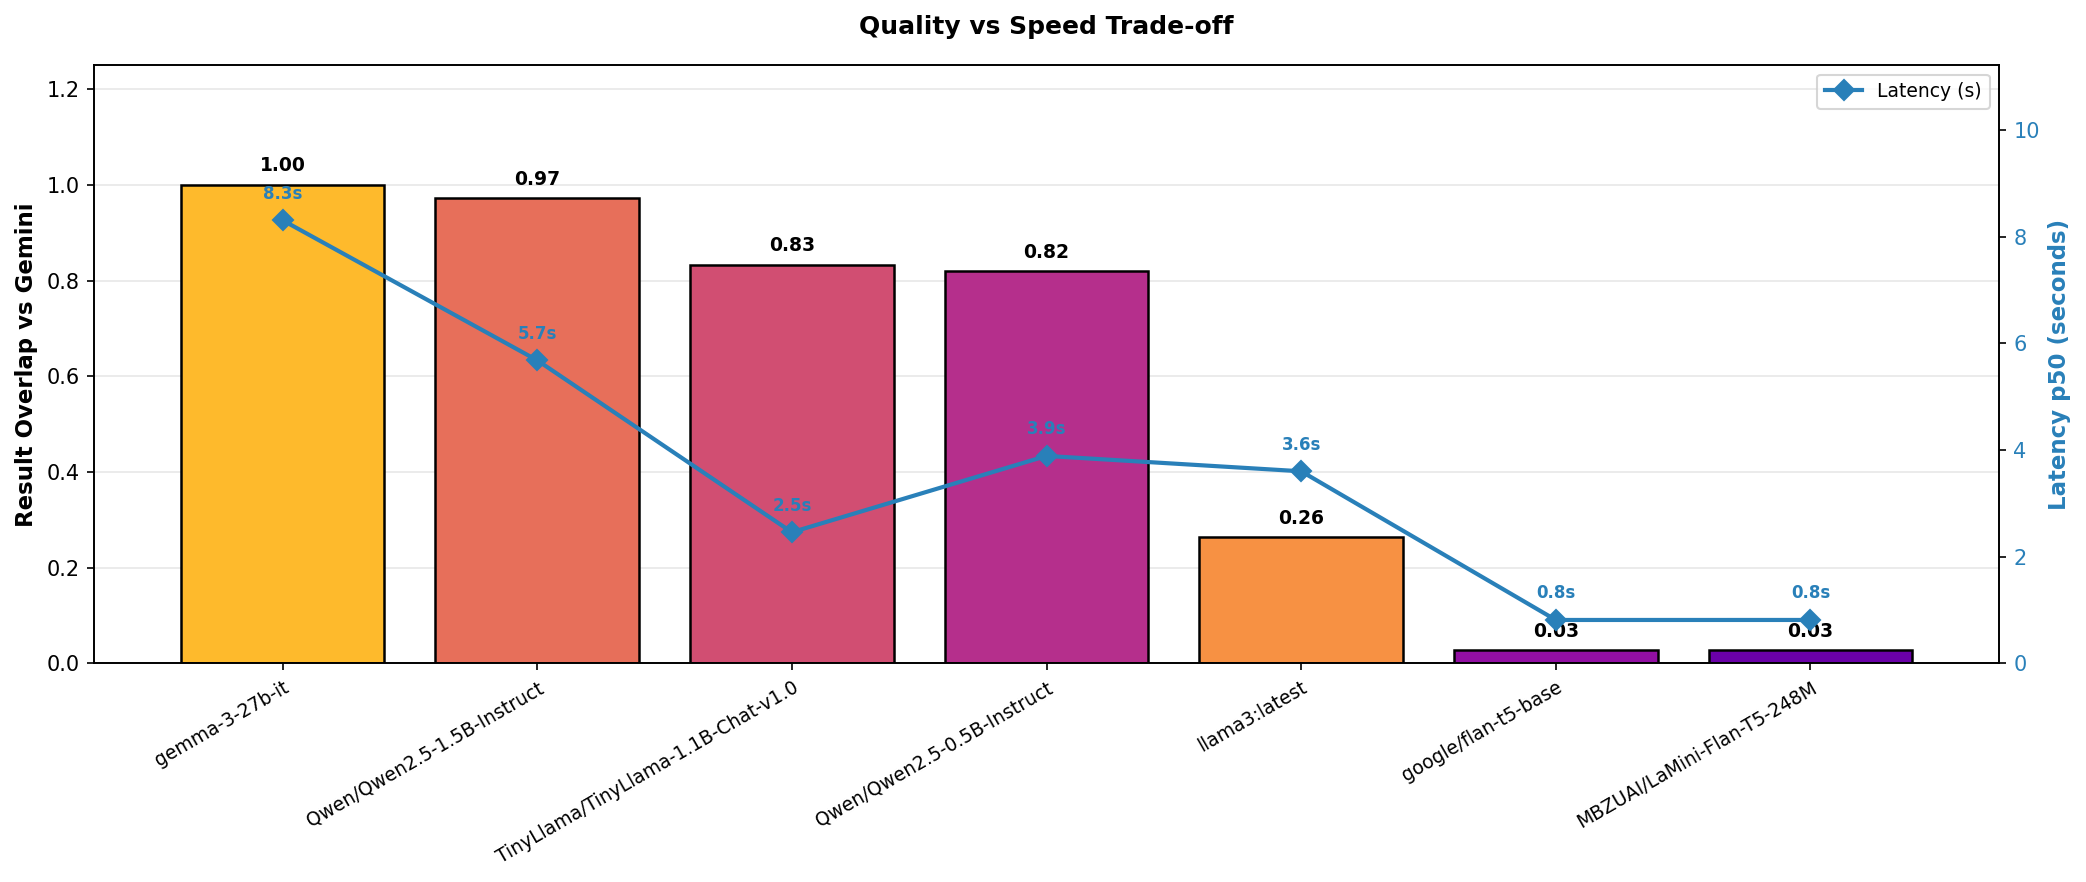
\includegraphics[width=\columnwidth]{../figures/correctness/temporal/fig4_quality_vs_speed.png}
    \caption{Temporal-suite quality-vs-speed trade-off. Bars show retrieval overlap with the Gemini baseline (left axis); the line shows mean latency in seconds (right axis). Models are sorted by quality. Qwen 1.5B and Gemini achieve the highest overlap; T5-family models are the fastest but produce no useful temporal output. Note: the quality axis reflects Jaccard overlap with Gemini's retrieved event set, not direct extraction accuracy.}
    \label{fig:quality_vs_speed}
\end{figure}

\section{Conclusion}
\label{sec:conclusion}

We report a systematic efficiency study on model-size minimization for event query grounding in the Curia campus search system. Across temporal and robustness suites, results confirm asymmetric degradation between keyword expansion and temporal grounding, plus meaningful backend sensitivity under perturbed queries. The best cross-suite local balance in our runs is Qwen 1.5B, while Qwen 0.5B remains a latency-oriented alternative that still passes robustness correctness gates.

Key findings:
\begin{itemize}
    \item \textbf{Task divergence is consistent}: Higher keyword F1 does not imply stronger temporal grounding; the two capabilities must be evaluated separately.
    \item \textbf{Usability threshold is dataset-dependent}: The 250M-class T5-family runs are non-usable on both suites, while robustness further narrows gate-passing models.
    \item \textbf{Stability is not purely a size effect}: Tail latency and error behavior vary by model/back-end pair; selected smaller models show heavy p95/max spikes.
    \item \textbf{Best practical operating point}: Qwen 1.5B provides the strongest cross-suite balance of correctness and latency, with Qwen 0.5B as a faster but lower-margin option.
    \item \textbf{Fallbacks remain limited}: Rule-based fallbacks recover explicit strings but do not fix semantically incorrect temporal reasoning in otherwise parseable JSON.
\end{itemize}

\subsection{Future Work}

\begin{itemize}
    \item \textbf{Quantized local models}: GGUF int4/int8 variants of Qwen2.5-1.5B and Qwen2.5-3B to improve the local accuracy-latency frontier without full-precision CPU inference.
    \item \textbf{Confidence-gated fallback}: Use token log-probabilities to decide when to trust LLM output versus fall back to rules, reducing unnecessary fallback invocations.
    \item \textbf{Recurring event queries}: Extend temporal extraction to handle recurring expressions (``every Monday'', ``weekly seminars'').
    \item \textbf{Expanded benchmark}: Add typo-robustness and cross-domain query variants; add a retrieval evaluation dataset with labeled relevant events to enable end-to-end hit-rate measurement currently unavailable due to corpus constraints.
\end{itemize}

\bibliographystyle{IEEEtran}
\bibliography{references}

\end{document}
